\documentclass{report}
\usepackage{amsmath, amssymb}
\usepackage[T1]{fontenc}
\usepackage{tgbonum}
\usepackage[spanish]{babel}
\usepackage{graphicx}
\usepackage[margin=1.25in]{geometry}
\graphicspath{{images/}}

\usepackage{titlesec}
\newcommand\secformat[1]{%
	\parbox[b]{.5\textwidth}{\filleft\bfseries #1}%
	\quad\rule[-12pt]{2pt}{70pt}\quad
	{\fontsize{60}{60}\selectfont\thesection}}
\titleformat{\section}[block]
{\filleft\normalfont\sffamily}{}{0pt}{\secformat}
\titlespacing*{\section}{0pt}{*3}{*2}[1pc]


\begin{document}
	
	\section{El temporizador\\ 555}
	
	El temporizador 555 es un dispositivo versátil y muy utilizado, porque puede ser configurado de dos modos distintos, bien como multivibrador monoestable o como multivibrador astable (oscilador). Un multivibrador astable no tiene estados estables y varía (oscila), por tanto, una y otra vez entre dos estados inestables, sin utilizar un circuito de disparo externo.

	\begin{figure}[h]
		\centering
		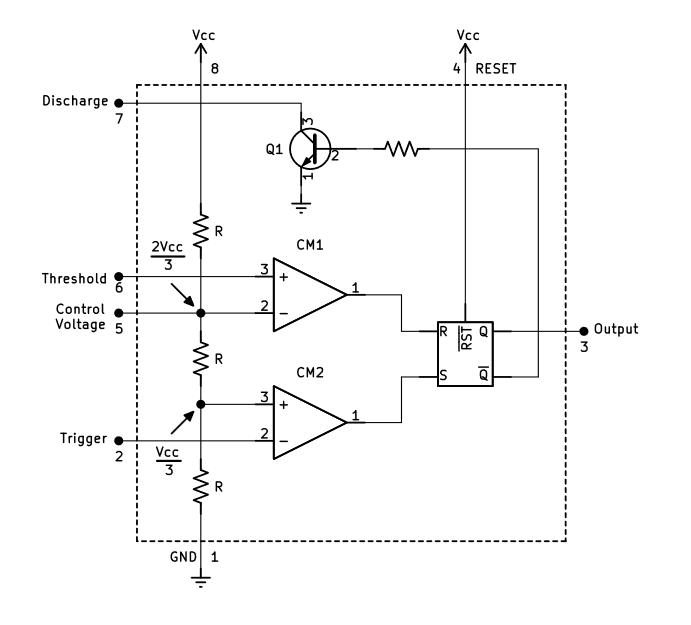
\includegraphics[scale=0.7]{diagrama_interno}
		\caption{Diagrama interno del temporizador 555.}
		\label{fig:1}
	\end{figure}
	
	\section{Funcionamiento básico}
	
	El diagrama de bloques del 555 se muestra en la figura \ref{fig:1}. el \textit{timer} consiste de dos comparadores $CM_1$ y $CM_2$, un $latch$ $RS$, un transistor de descarga $Q_1$ y una red divisora de voltaje.
	
	\subsection{El comparador}
	
	Los comparadores (figura \ref{fig:2}) son dispositivos cuyas salidas están en un nivel ALTO cuando la tensión de entrada positiva (+) es mayor  que la tensión de entrada negativa. y está a un nivel BAJO cuando la tensión de entrada negativa es mayor que la tensión de entrada positiva. Matemáticamente, el voltaje de saluda de un comparador está dado por:
	
	\begin{figure}[h]
		\centering
		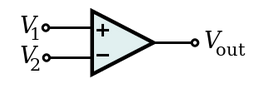
\includegraphics[scale=0.7]{comparador}
		\caption{Símbolo del comparador}
		\label{fig:2}
	\end{figure}
	
	\begin{align}
		V_o = 
		\begin{cases}
			+V_{cc}, & \text{if } V_1>V_2\\
			-V_{cc}, & \text{if } V_1<V_2
		\end{cases}
	\end{align}
	
	\subsection{Divisor de tensión}
	El divisor de voltaje de la figura \ref{fig:3} compuesto por tres resistencias establecen el voltaje en la terminal inversora de $CM_1$ a $2V_{cc}/3$ y un voltaje en la terminal no inversora de $CM_2$ de $V_{cc}/3$.
	
	\begin{figure}[h]
		\centering
		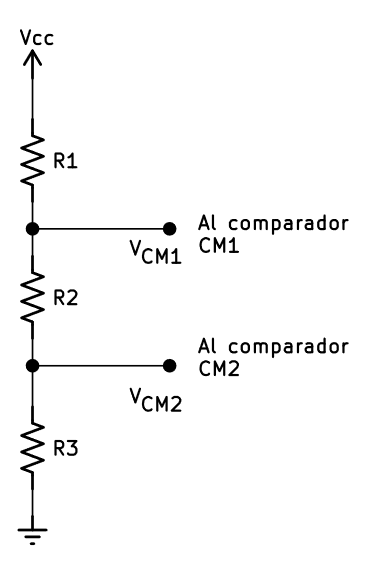
\includegraphics[scale=0.7]{divisor}
		\caption{Red divisora de voltaje interna del timer 555}
		\label{fig:3}
	\end{figure}

	el voltaje a través de $R_3$ establece un voltaje de $V_{cc}/3$ en la terminal positiva del comparador $CM_2$, para comprobarlo, usamos el principio de división de voltaje obtenido:
	
	\begin{align}
		V_{CM2} = \frac{R_3 V_{cc}}{R_1 + R_2 + R_3}
	\end{align}
	
	Asumiendo que $R_1 = R_2 = R_3 = R$ obtenemos
	
	\begin{align}
		V_{CM2}=\frac{R}{3R} V_{cc} \nonumber
	\end{align}

	o bien
	
	\begin{align}
		V_{CM2}=\frac{1}{3} V_{cc} 
	\end{align}

	En la figura se observa el diagrama esquematico del integrado 555, podemos apreciar la red divisora de voltaje la cual está conectada a os dos comparadores, esta red de tres resistencias tiene valores idénticos (de $5k\Omega$), por lo que se dice que de ahí surgió su famoso nombre.\\
	
	Ahora, el voltaje a través de la terminal negativa de $CM_1$ está dado por 
	\begin{align}
		V_{CM1} = \frac{R_2 + R_3}{R_1 + R_2 + R_3} V_{cc}
	\end{align} 
	
	De nueva cuenta, dado que $R_1 = R_2 = R_3 = R$ 
	
	\begin{align}
		V_{CM1} = \frac{2}{3} V_{cc}
	\end{align} 
\end{document}